\documentclass{article}

\usepackage[margin=2.5cm,left=2cm,includefoot]{geometry}
\usepackage{hyperref}
\usepackage{array}
\usepackage{enumitem}
\usepackage{graphicx}
\usepackage[section]{placeins}
\usepackage{titlesec}
\usepackage{float}

% Set depth for sections (one more than usual)
\setcounter{secnumdepth}{4}

% Set paragraphs to be the 4th section depth
\titleformat{\paragraph}
{\normalfont\normalsize\bfseries}{\theparagraph}{1em}{}
\titlespacing*{\paragraph}
{0pt}{3.25ex plus 1ex minus .2ex}{1.5ex plus .2ex}

% Header and footer
\usepackage{fancyhdr}
\pagestyle{fancy}

\rhead{COS301 - \LaTeX}
\lhead{Team Algol}
\fancyfoot{}
\fancyfoot[R]{Page \thepage}

\renewcommand{\headrulewidth}{2pt}
\renewcommand{\footrulewidth}{1pt}
%

\begin{document}

	\begin{titlepage}
		\begin{center}

			\begin{figure}
				
\includegraphics[width=\linewidth]{logo.jpg}	
			\end{figure}

			\line(1,0){400}\\
			[6mm]
			\huge{
				\bfseries Architectural Requirements Specifications and Design
			}\\
			[2mm]
			\line(1,0){300}\\
			[10mm]
			\textsc{\large NavUP}\\
			[7.5mm]
			\textsc{\large University of Pretoria - Team Algol}\\
			[10mm]
			\large{\textbf{Created By:}}\\
			[2mm]
			% Add your own details here 
			\href{https://github.com/KeatonPennels}{Keaton Pennels - 14373018}\\
			\href{https://github.com/Chris19951225}{Hristian Vitrychenko - 15006442}\\
      \href{https://github.com/lindelo}{Lindelo Mapumulo - 12002862}\\
			\href{https://github.com/DuartBreedt}{Duart Breedt - 15054692}\\[5mm]


		\href{https://github.com/Chris19951225/COS-301-Team-Algol}{\textsc{\Large GitHub Repository - Team Algol}}
		\\
		\href{https://github.com/Chris19951225/COS-301-Team-Algol}{\textsc {For more information, please click here}}
		  
		\end{center}
		\begin{flushright}
			\textsc{\large 26 February 2017}
		\end{flushright}
	\end{titlepage}

	\cleardoublepage
	\thispagestyle{empty}
	\tableofcontents
	\cleardoublepage

	\thispagestyle{empty}
	\listoffigures
	\cleardoublepage
	\setcounter{page}{1}
	
	
	\section{Introduction}\label{sec:intro}
		This chapter of the document aims to identify the architectural design specifications which satisfy the identified functional requirements of the NavUP system. Additionally, it will include any terms, abbreviations, acronyms and references used throughout this document.
	
		\subsection{Purpose}\label{subsec:purpose}
			The main purpose of this document is firstly identifying the subsystem architectural design requirements, constraints, integration need  and then addressing these elemts by using architectural patterns and diagrams to model system behaviour and interactions. The choice of appropriate technologies for the implementation of this system that satisfy the various requirements will also be prosposed along with motivations for these propositions 
				
		\subsection{Definitions, Acronyms, and Abbreviations}\label{subsec:daa}
			\begin{table}[h!]
				\centering
				\caption{Table of Definitions, Acronyms, and Abbreviations used in this document}
				\label{tab: Table 1}
				\begin{tabular}{| m{4cm} | m{12cm} |}
					\hline
					\textbf{Term} & \textbf{Definition} \\
					\hline
					SCALE & Scale to measure the requirement \\
					\hline
					METER & Location of the requirement on the scale  \\
					\hline
					MUST & Mandatory requirement to ensure good system performance \\
					\hline
					WISH & Preferred requirement to ensure good system performance \\
					\hline
					
				\end{tabular}
			\end{table}
	
		\subsection{References}\label{subsec:references}
		List each document referenced in the SRS by title, report number, date, publisher, and where and how to get it
		
	\section{Requirements and Constraints}\label{sec:requirements}

	The following section provides all the requirements of NavUP, and possible constraints regarding the mobile application.
			\subsection{External Interface Requirements}\label{subsec:external}
			This section provides a detailed description of all the inputs and outputs of the system. Descriptions of the user, hardware, software and communication interfaces are also provided.
			\subsubsection{User interfaces}
			Upon opening the application, a first time user (or a user that had logged out) should see the splash page - Figure 1. The splash page will allow a user to continue as a guest (without logging in) or login in as a user. The user can either swipe left to login or right to use the application as a guest. 
			If a user chooses to use NavUP as a guest, then they are directed to a landing page. The landing page includes an interactive list of all the features (e.g. Location Access, Route Access, Profile Information)in NavUP. \\
			
			The log in page (Figure 2) should prompt the user to enter their login details (user name \& password). If the user has not yet created an account, they will be prompted to register a new account before they can use or continue with the application. 
			The user register page bears resemblance to the login page prototype, but includes input fields for the user's email address and two password fields (one for the actual password, and another to verify the previously entered password). The chosen username should not be an existing one, and should also not be longer than 15 alphanumeric characters). The user's password needs to be at least eight characters, and must include at least one number. \\
			
			In addition to being able to register as a new user, a user should be able to view, update and/or delete their profile. The prototype of this page is shown on Figure 3; on this page, a user can perform CRUD operations (excluding CREATE) on their profiles. Admin profiles will have additional options (e.g. making a normal user an administrator user). These options will appear in the "User Details" page.
\begin{figure}[H]
    \minipage{0.32\textwidth}
	\centering{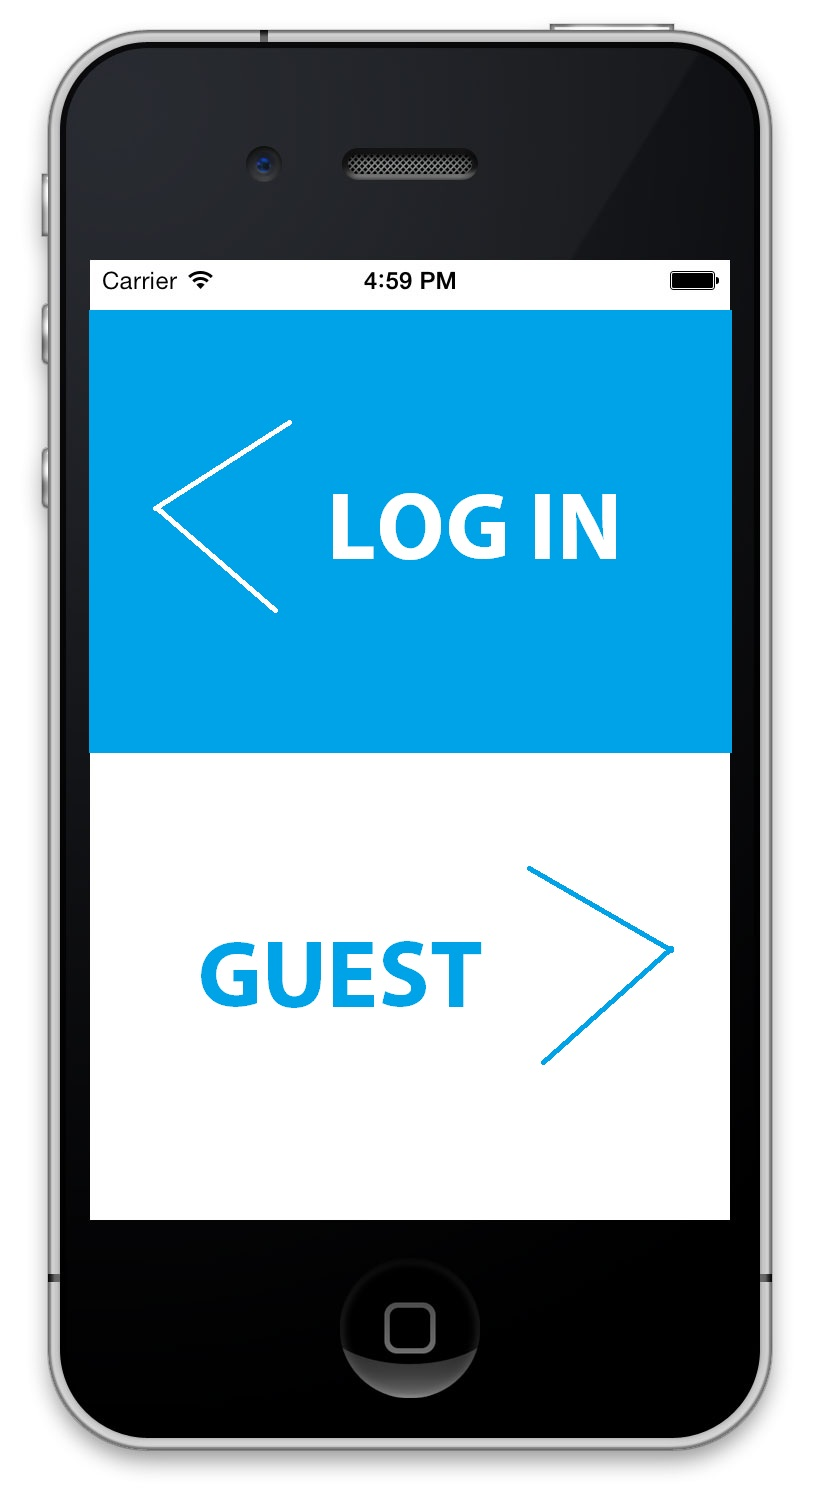
\includegraphics[width=0.5\linewidth]{./images/Splash_Screen.JPG}}
	\caption{Splash Screen}
	\endminipage\hfill
	\minipage{0.32\textwidth}
	\centering{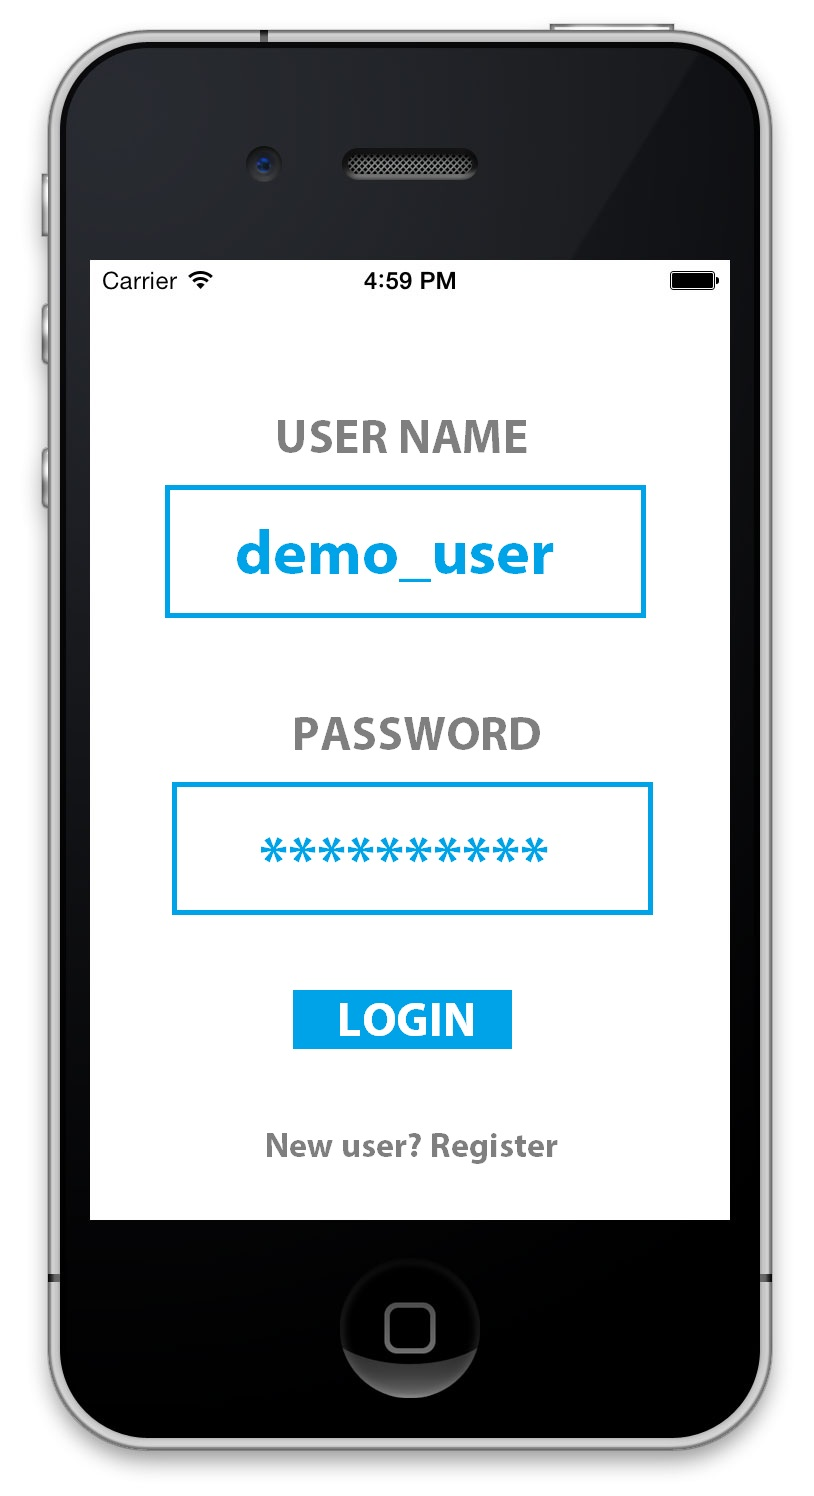
\includegraphics[width=0.5\linewidth]{./images/Login_Screen.JPG}}
	\caption{Login Screen}
	\endminipage\hfill
	\minipage{0.32\textwidth}
	\centering{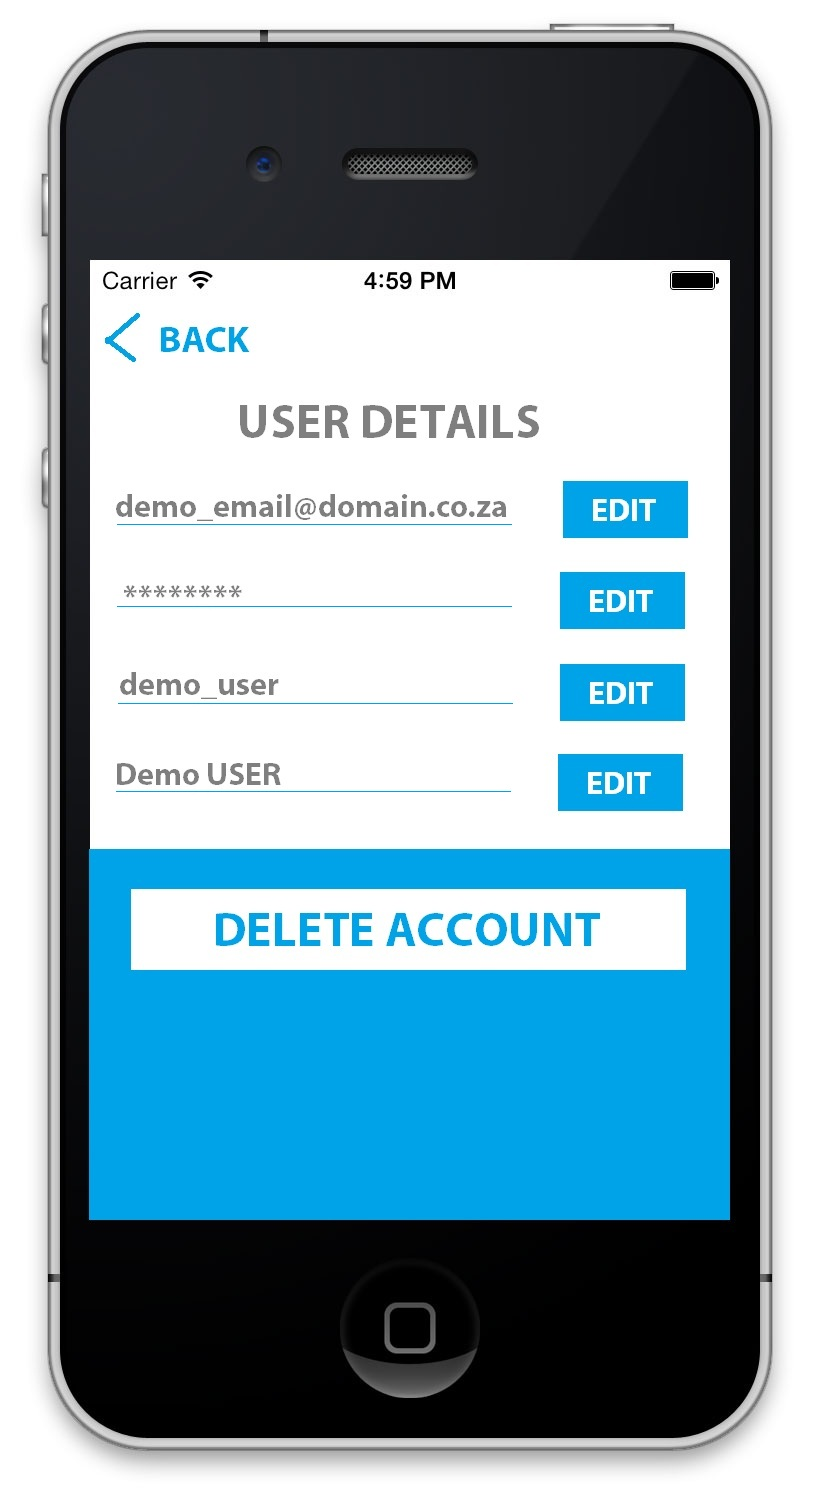
\includegraphics[width=0.5\linewidth]{./images/User_Details.JPG}}
	\caption{User Details Screen}
	\endminipage\hfill
\end{figure}

A user should be able to find the directions between two (or more) points by entering the name of the points. The user should also be provided with additional features to improve the navigation between these points, these include but are not limited to the shortest route and the simplest route. Figure 4 shows the search page to find directions between two points, and Figure 5 shows the results and further filtering options to improve the nature of the directions.\\

\begin{figure}[H]
    \minipage{0.3\textwidth}
	\centering{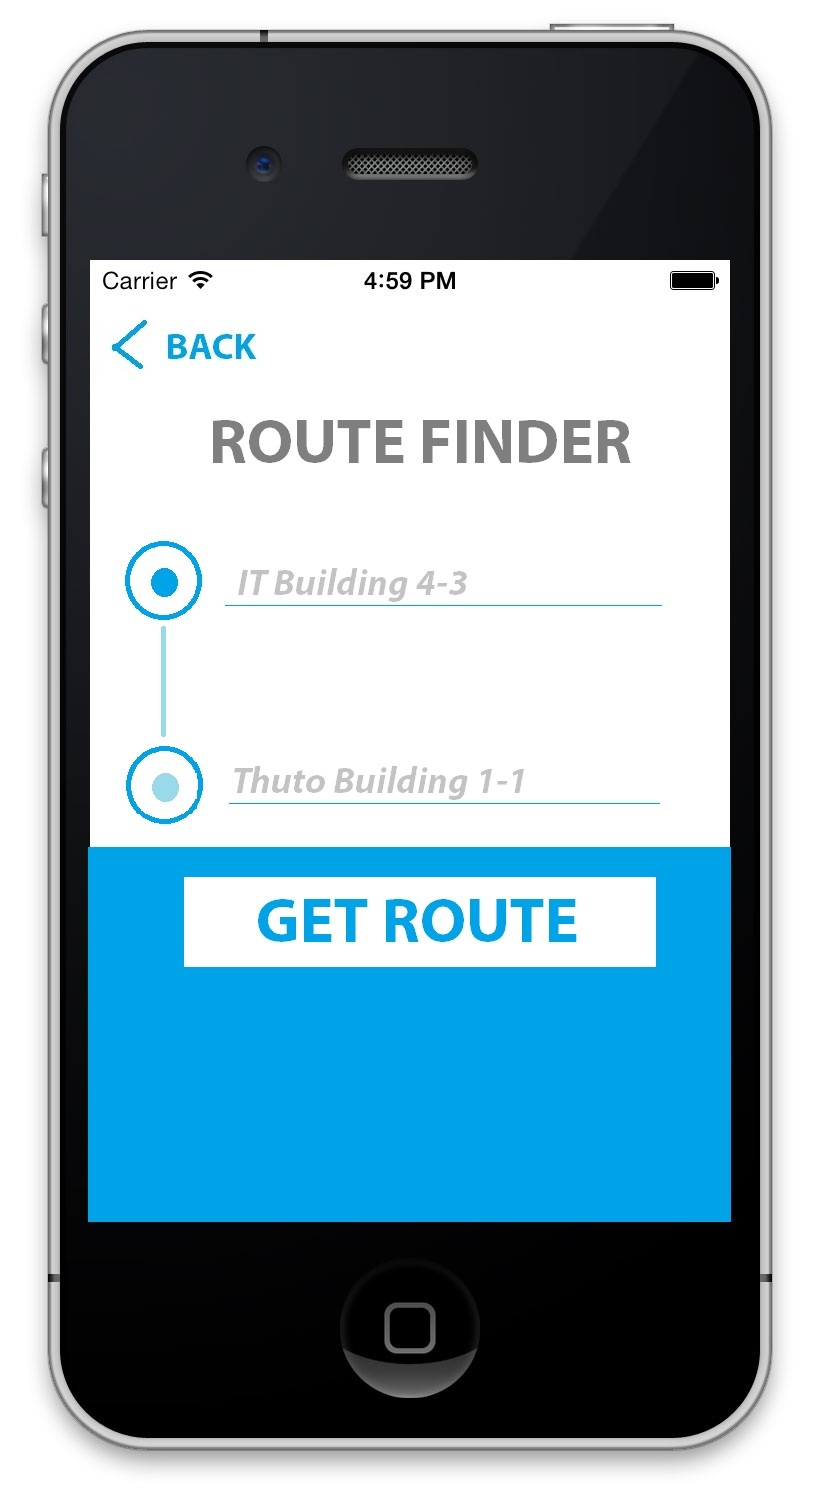
\includegraphics[width=0.5\linewidth]{./images/Get_Directions_Search.JPG}}
	\caption{Get Directions Search Screen}
	\endminipage\hfill
	\minipage{0.3\textwidth}
	\centering{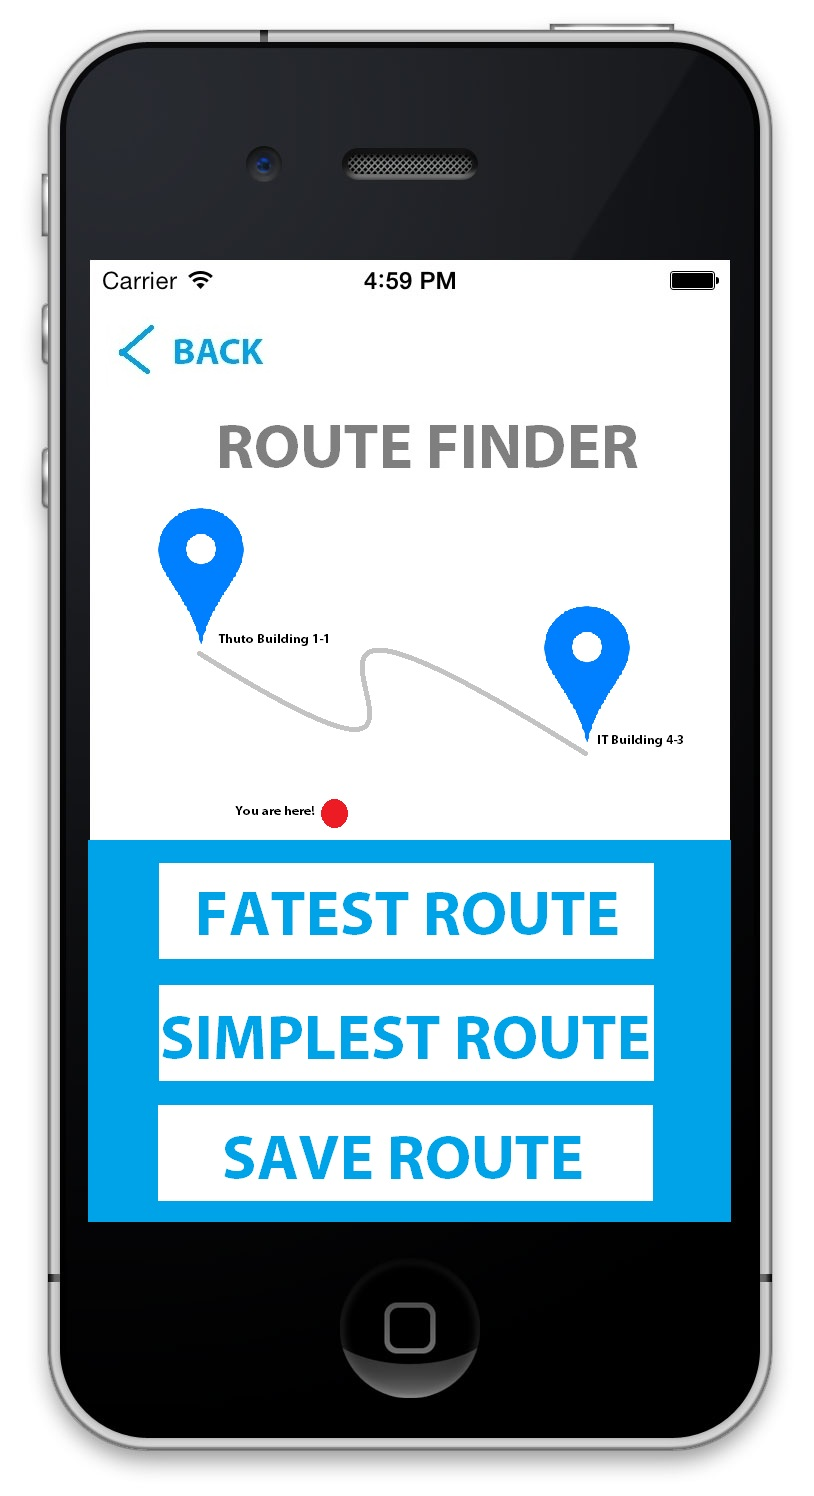
\includegraphics[width=0.5\linewidth]{./images/Get_Directions_Results.JPG}}
	\caption{Get Directions Result Screen}
	\endminipage\hfill
	\minipage{0.3\textwidth}
	\centering{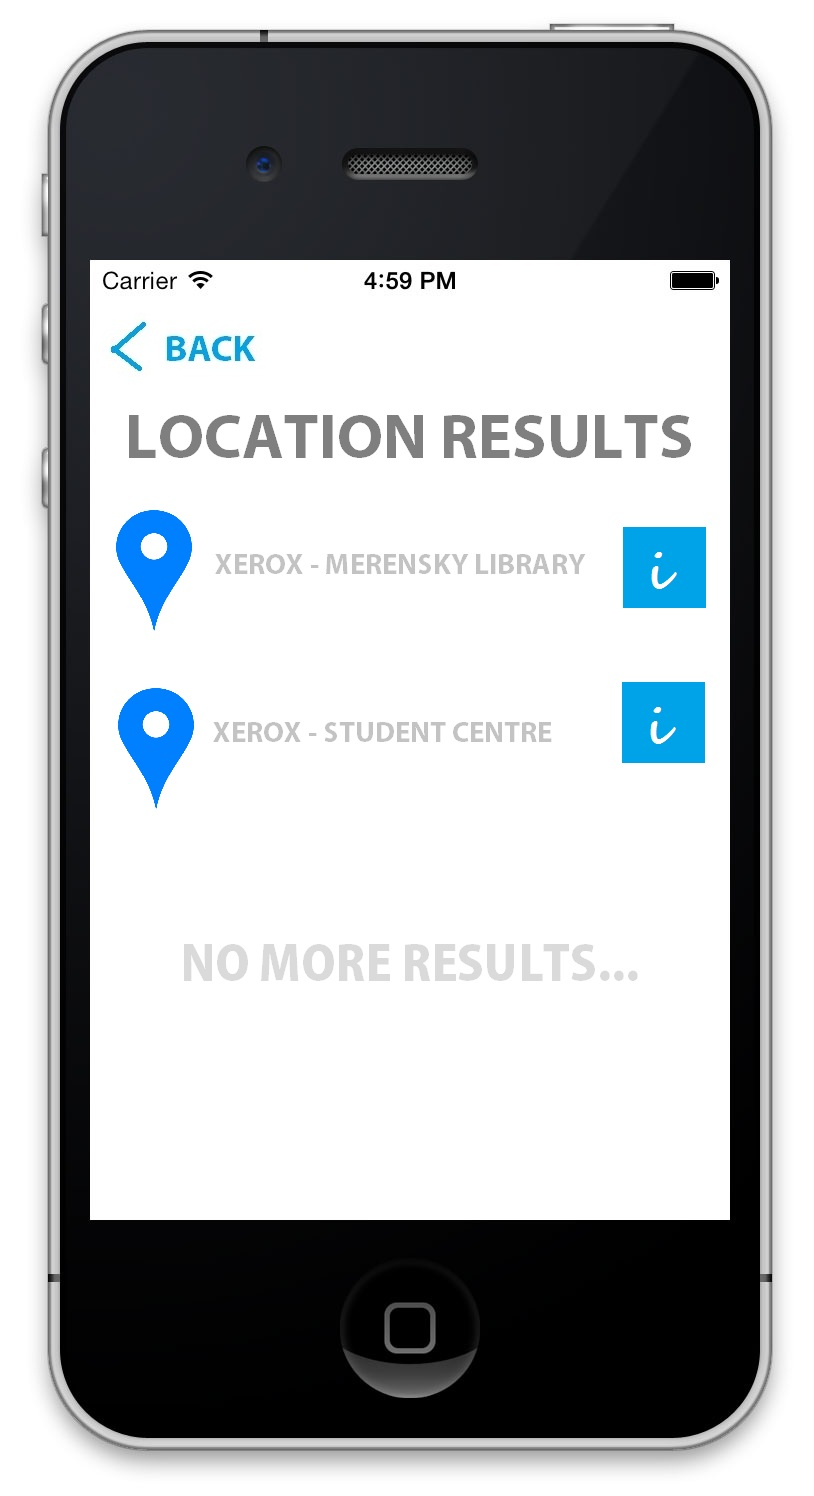
\includegraphics[width=0.5\linewidth]{./images/POI_Results.JPG}}
	\caption{Search Locations Result(s) Screen}
	\endminipage\hfill
\end{figure}

Users should also be able to get their current location, save various points of interest and search for a location. Figure 6 shows the prototype page for the results produced after a user has searched for a location. \\

A user should also be able to send a notification. The notification page should have a similar layout as the other pages shown across Figure 1 - 6. The body of the notification should not be longer than 140 characters.

The web-based component of NavUP should be similar to the mobile-based component. The layout, however, should be relevant to a web-only device. Features such as sliding left or right should be replaced by appropriate gestures.
			\subsubsection{Hardware interfaces}
			Since NavUP uses existing hardware (i.e. smart devices), it does not require direct hardware interfaces other than the interfaces that are provided by the user's device. The GPS features are explicitly managed by the user's device, particularly the operating system on which the device runs.
			\subsubsection{Software interfaces}
			NavUP communicates with the device's GPS to get data about the user's location and the other geographical information regarding the user's location. Furthermore, the application communicates with the on-campus wireless hotspots to tag the relative location of a user within a building. NavUP will mostly just perform read operations, which are communicated to the application via the device's operating system.
			\subsubsection{Communication interfaces}
			The application will be heavily dependent on the device's GPS; without this communication NavUP will be unable to perform any location specific operations (including getting the user's current location). The application also needs a working wireless network connection in order to facilitate communication with the GPS's remote database. The wireless hotspots within the university will also be required to get the user's relative building location; without this, it may be difficult to provide accurate results.

			\subsection{Performance Requirements}\label{subsec:performance}
				This section provides a detailed specification of the user's interaction with NavUP, as well as the measures put in place to ensure good system performance.
			
			\subsubsection{Intuitive user interface}
		    \begin{itemize}
		    \item[]TITLE      : Intuitive user interface
		    \item[]DESCRIPTION: The user interface for NavUP should be intuitive and not at any stage confuse users.
		    \item[]RATIONAL   : This ensures easy navigation for the user when using NavUP.
		    \item[]DEPENDENCY : No dependencies.
		    \end{itemize}
			\subsubsection{Intuitive search feature}
			\begin{itemize}
		    \item[]TITLE      : Intuitive search feature
		    \item[]DESCRIPTION: The user should be provided with clear search results when trying to find locations.
		    \item[]RATIONAL   : This ensures that users are not confused by the search results, and can understand the details returned by the search results.
		    \item[]DEPENDENCY : No dependencies.
		    \end{itemize}	
			\subsubsection{Intuitive map view}
			\begin{itemize}
		    \item[]TITLE      : Intuitive map view
		    \item[]DESCRIPTION: The map view presented to the user should be easy to understand and leave no room for ambiguous interpretations.
		    \item[]RATIONAL   : This ensures that the user will be able to use the map view to navigate effectively.
		    \item[]DEPENDENCY : No dependencies.
		    \end{itemize}	
			\subsubsection{Intuitive information/help feature}
			\begin{itemize}
		    \item[]TITLE      : Intuitive information/help feature
		    \item[]DESCRIPTION: The information buttons (seen in the search results) - and help features - should be easy to find and use.
		    \item[]RATIONAL   : This ensures that users can use information and help features easily, since the users are most likely to interact with these features when using NavUP for the first time.
		    \item[]DEPENDENCY : No dependencies.
		    \end{itemize}	
			\subsubsection{Fast response time}
			\begin{itemize}
		    \item[]TITLE      : Fast response time
		    \item[]DESCRIPTION: Results for getting routes or finding locations should not take much time.
		    \item[]SCALE      : The time it takes to get a route and find a location.
		    \item[]METER      : Measured by finding 100 routes and locations, during the testing phase.
		    \item[]MUST       : Must take no more than 3 seconds 100\% of the time.
		    \item[]WISH       : Preferably shouldn't take longer than a second, 100\% of the time.  
		    \end{itemize}
			\subsubsection{Dependable system}
			\begin{itemize}
		    \item[]TITLE      : Dependable system
		    \item[]DESCRIPTION: NavUP should be able to deal with (recover from) all faults.
		    \item[]SCALE      : Should a user incorrectly enter search criteria or NavUP not be able to establish an internet connection, a notification should be sent to a user.
		    \item[]METER      : Measured by using NavUP for at least 10 hours, during the testing phase.
		    \item[]MUST       : NavUP must be dependable at all times.
		    \end{itemize}	
						
			\subsection{Design Constraints}\label{subsec:design constraints}	
				This section provides the design constraints on NavUP's software, which is caused by the device's hardware.
				
		    \subsubsection{Hard disk drive space}
			\begin{itemize}
		    \item[]TITLE      : Hard disk drive space
		    \item[]DESCRIPTION: The amount of space NavUP occupies on installation.
		    \item[]SCALE      : Megabyte(MB).
		    \item[]METER      : Monitoring the space occupation (in megabytes) during the testing phase.
		    \item[]MUST       : NavUP shouldn't occupy more than 100MB.
		    \item[]WISH       : Preferably, NavUP shouldn't occupy more than 50MB.
		    \end{itemize}
		    
		    \subsubsection{Application RAM (Random-Access-Memory) usage}
			\begin{itemize}
		    \item[]TITLE      : Application RAM (Random-Access-Memory) usage
		    \item[]DESCRIPTION: The amount of RAM NavUP uses while running on the device. 
		    \item[]SCALE      : Megabyte (MB).
		    \item[]METER      : Monitoring RAM usage (in megabytes) during the testing phase.
		    \item[]MUST       : NavUP shouldn't use more than 50MB of the device's RAM.
		    \item[]WISH       : Preferably, NavUP shouldn't use more than 30MB of the device's RAM.
		    \end{itemize}
			\subsection{Software System Attributes}\label{subsec:attributes}
			This section provides descriptions for the quality requirements: security, maintainability, availability, usability and scalability.
			
			\subsubsection{Security}
			Security is currently not a top priority for NavUP since the biggest threat is unauthorized access to users' geographical data within the university. However, this data should still be kept confidential via encryption. Users should be authenticated to ensure that they do not have unauthorized access to other users' profiles and/or administration privileges.
			 
			\subsubsection{Maintainability}
			The technologies used for NavUP should be relevant and expected to be relevant for the longest possible time. Software Developers that were not involved in the initial development process should be able to understand the system in order to improve the software. This is very necessary when new features are required and/or depleted features need to be removed.
			
			\subsubsection{Availability}
			NavUP should always be available, especially during "peak-usage" times like the beginning of every academic year and Open Day. Addition/removal of features should not affect the availability of NavUP. Finally, NavUP shouldn't have a single point-of-failure; the application should continue functioning even if one or more feature(s) fail.
			
			\subsubsection{Usability}
			Since users with different technological backgrounds are expected to use NavUP, the user interface (UI) needs to conform to good UI design standards. The system should never at any point confuse users, and should be as interactive as possible.
			Usability tests need to be performed on users with different technological backgrounds to find any issues with the general front-end design of NavUP. These problems should be addressed before deployment to ensure a fun and easy to use system. Finally, the system should cater for at least three most spoken languages by students/staff members of the university.
			
			\subsubsection{Scalability}
			NavUP has the potential of being used by over 50 000 students/staff members/guests. The system needs to be able to still function normally even when too many users are interacting with NavUP.
			
		\newpage

		\section{Module Design}\label{sec:moduels}	
      \subsection{User Management Subsystem}\label{subsec:users}
      	\begin{figure}[H]
			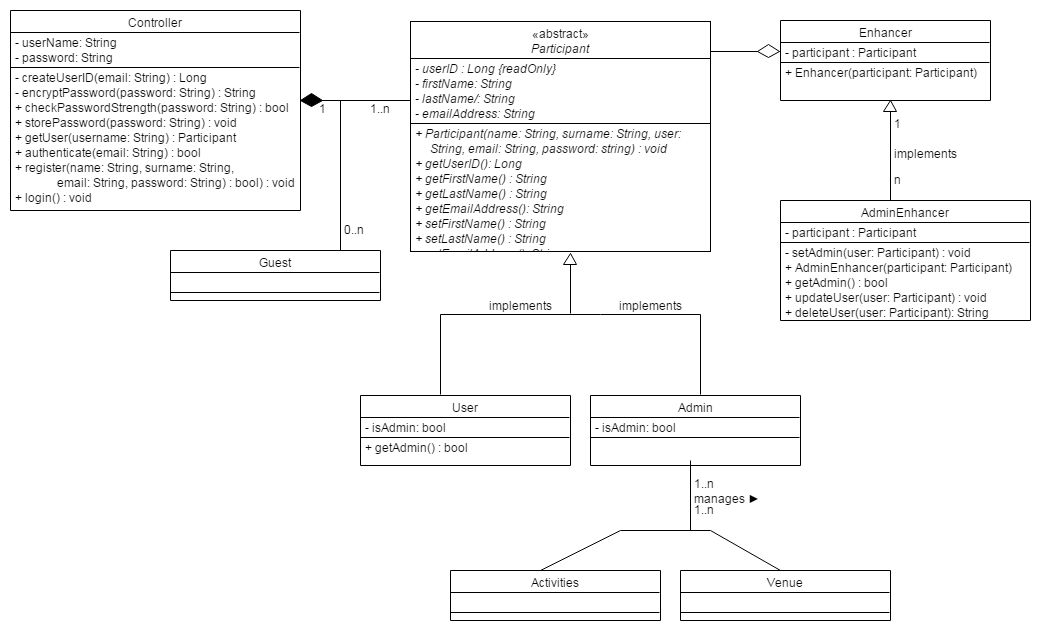
\includegraphics[scale=0.5]{Diagrams/User_Class_Diagram.png}
			\caption{User Management Model Class Diagram}
			\label{fig:User_class}
		\end{figure}
		
		The above diagram depicts a class diagram of the User Management Model. A The Participant class is a abstract class which defines the common attributes and methods associated with the two main personnel who will interact with NavUp, namely Users and Administrators, which are the concrete implementations of Participant.\\\\
			\subsection{Navigation Subsystem}\label{subsec:navigation}
			
			\subsection{Notification Subsystem}\label{subsec:notification}
			
				\begin{figure}[h!]
					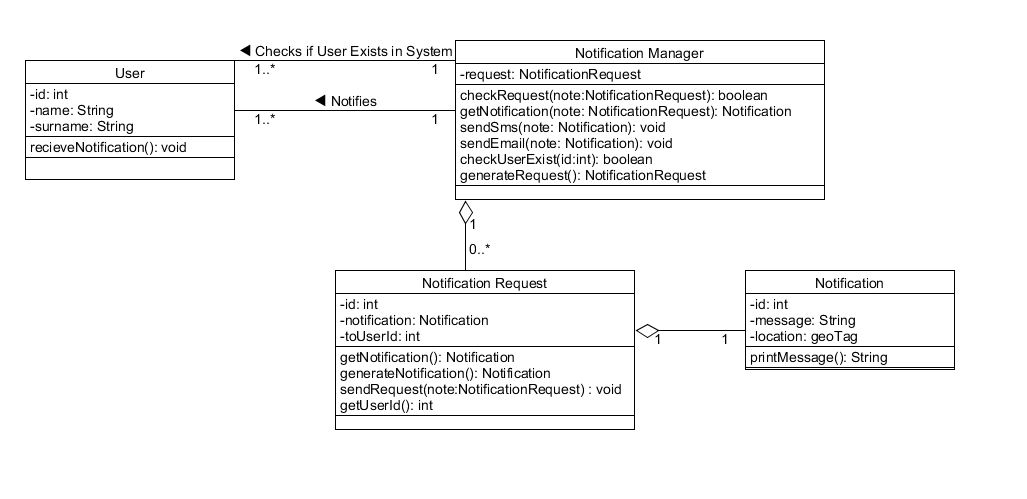
\includegraphics[scale=0.5]{./Diagrams/Class_Diagram_Notifications.JPG}
					\caption{Notifications Subsystem Class Diagram}	
				\end{figure}
			
				\begin{figure}[h!]
					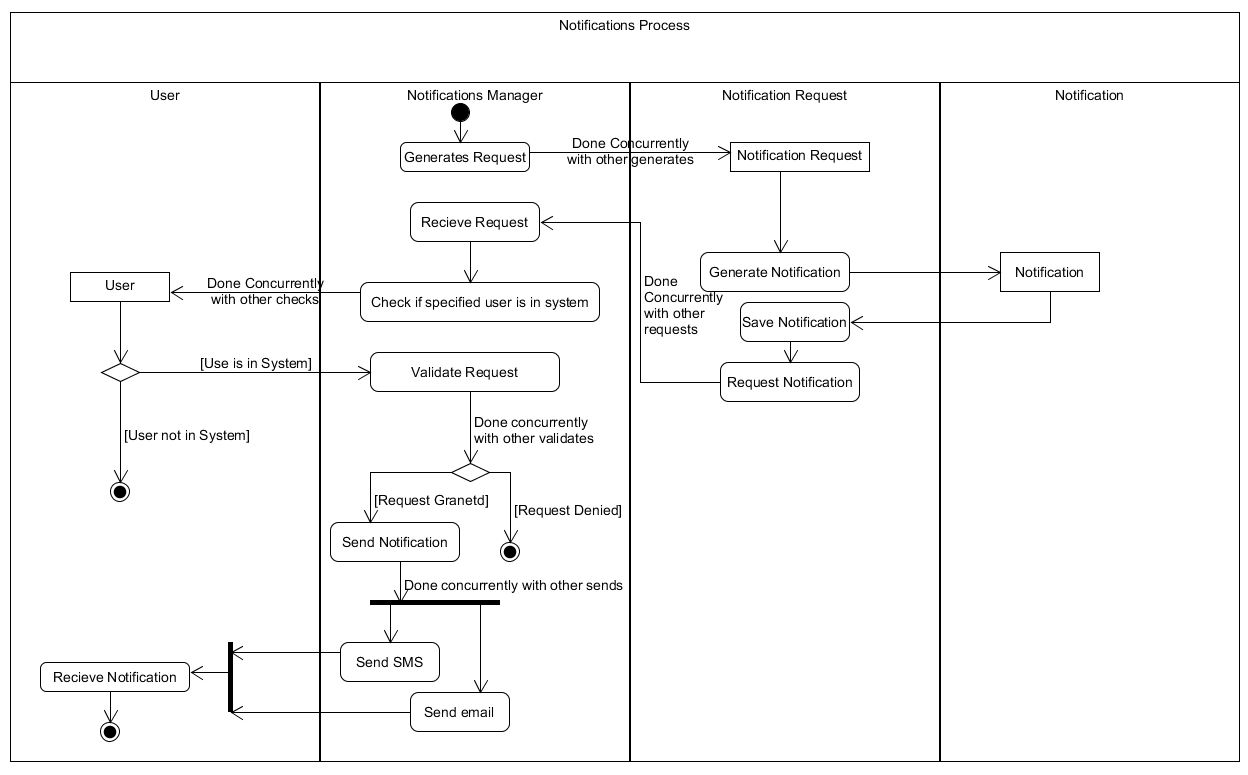
\includegraphics[scale=0.5]{./Diagrams/Activity_Diagram_Notifications.JPG}
					\caption{Natifications Subsystem Activity Diagram}	
				\end{figure}
				
				\begin{figure}[h!]
					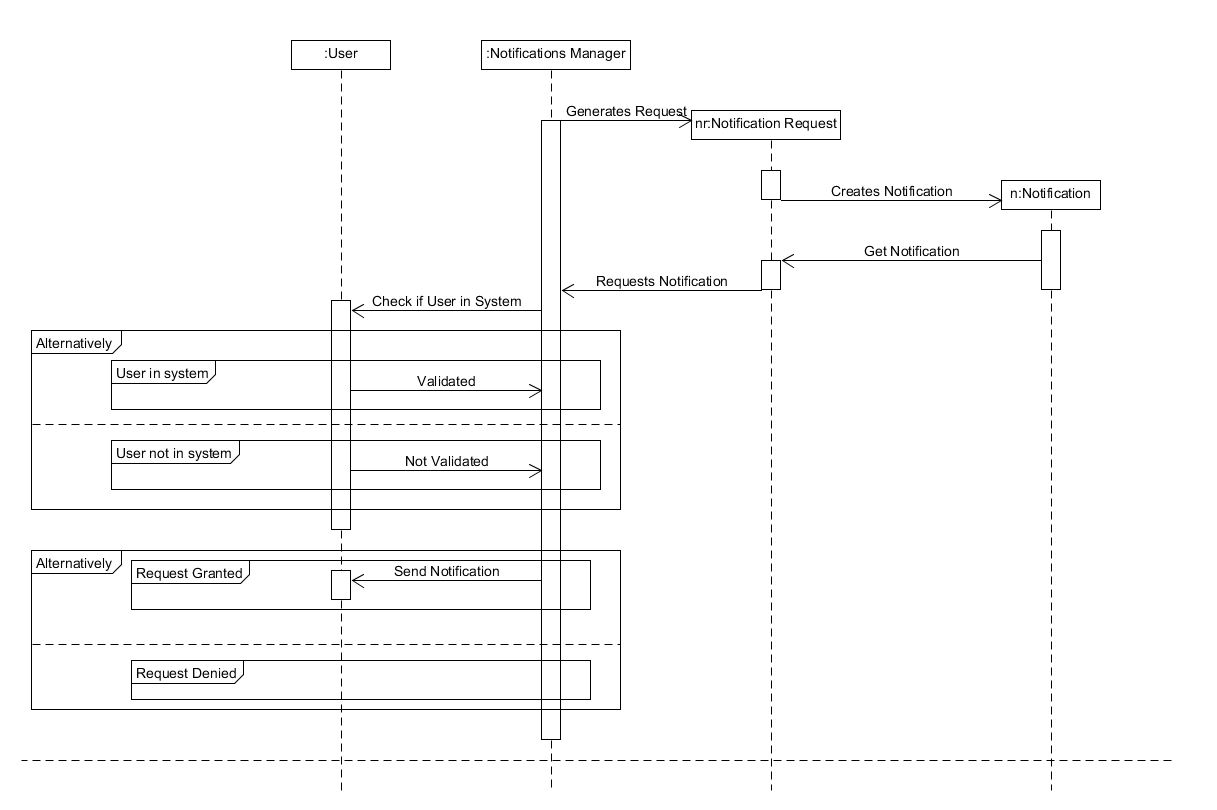
\includegraphics[scale=0.5]{./Diagrams/Sequence_Diagram_Notifications.JPG}
					\caption{Notifications Subsystem Sequence Diagram}	
				\end{figure}
				
				\begin{figure}[h!]
					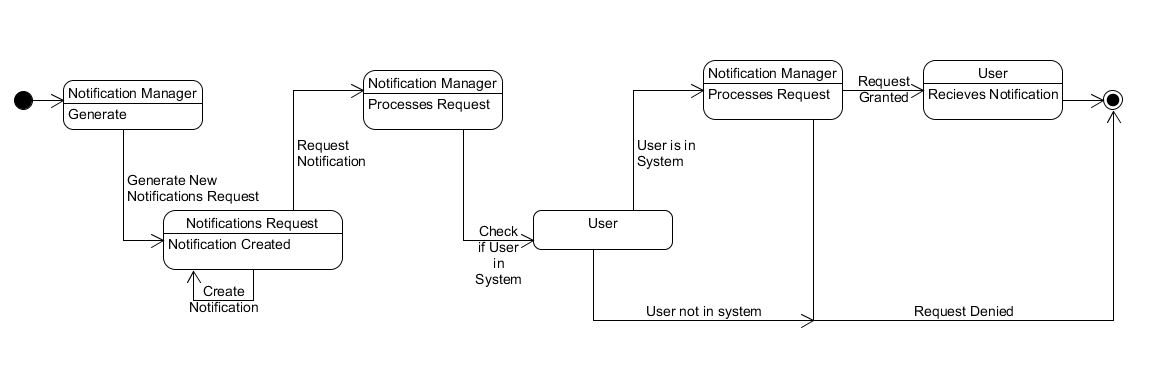
\includegraphics[scale=0.5]{./Diagrams/State_Diagram_Notifications.JPG}
					\caption{Notifications Subsystem State Diagram}	
				\end{figure}
				
				\begin{figure}[h!]
					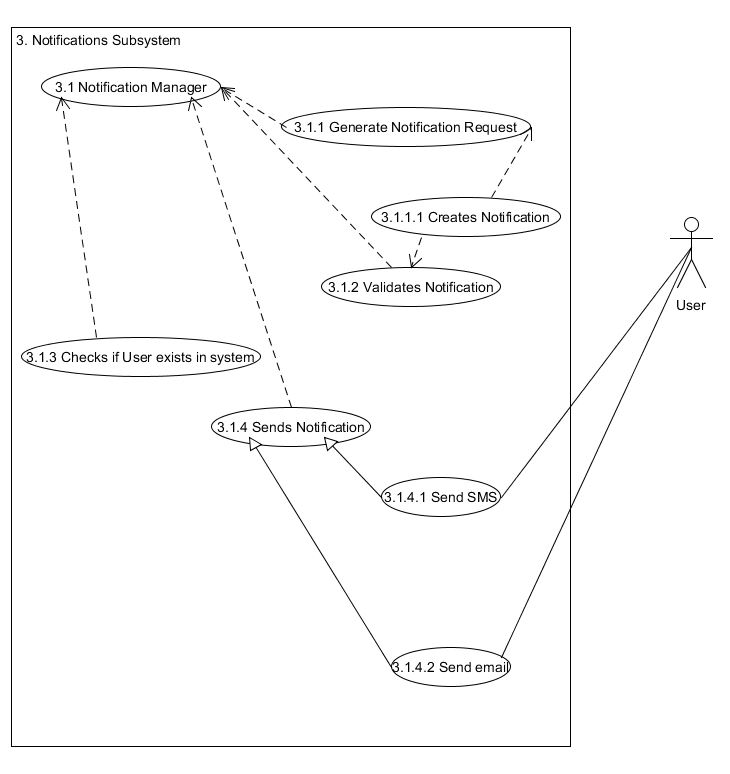
\includegraphics[scale=0.5]{./Diagrams/Use_Case_Diagram_Notifications.JPG}
					\caption{Notifications Subsystem Use Case Diagram}	
				\end{figure}
				
				\begin{figure}[H]
                     \includegraphics[height=0.8\textheight]{Navigation_State.png}
                     \caption{Route Access State Diagram}
					 \label{fig:navigation_state}
			    \end{figure}
			    
			    \begin{figure}[H]
                     \includegraphics[width=\textwidth]{Navigation_UseCase.png}
                     \caption{UseCase Diagram}
					 \label{fig:navigation_UseCase}
			    \end{figure}

			    
			\subsection{User Subsystem}\label{subsec:users}
			\subsection{Notification Subsystem}\label{subsec:notification}

			\newpage
			\subsection{Points of Interest Subsystem}\label{subsec:points of interest}
				\begin{figure}[H]
		 \includegraphics[height=0.8\textheight]{PoI_Class.png}
                     \caption{Point of Interest Class Diagram}
					 \label{fig:PoI_class}
			    \end{figure}

			\begin{figure}[H]
		 \includegraphics[height=0.8\textheight]{PoI_UseCase.png}
                     \caption{Point of Interest Use Case Diagram}
					 \label{fig:PoI_UseCase}
			    \end{figure}

		\newpage

		\section{System assessment}\label{sec:assessment }	
			\subsection{Technology choices}\label{subsec:tech choices}
			\subsection{Quality and Feasibility of Design}\label{subsec:quality}

	 \cleardoublepage
	 \section{Appendices}\label{sec:appendices}
 		
	


\end{document}
